% Computer Architecture (4190.308) Fall 2016 
% Seoul National University CARES Lab
% Lab 4 documentation

% Lines that need modification : 26~28, 145(ipcafter results), 152~153 (results), 249~262 (results)

\documentclass{article}
\usepackage{graphicx, caption, subcaption, verbatim, moreverb, alltt, kotex}
\usepackage[protrusion=true,expansion=true]{microtype}
\usepackage{fancyvrb}
\usepackage{hhline}
\usepackage{multirow}
\DeclareGraphicsExtensions{.pdf,.png,.jpg}
\let\verbatiminput=\verbatimtabinput

\setlength{\oddsidemargin}{0.25in}	% 1.25in left margin
\setlength{\evensidemargin}{0.25in}	% 1.25in left margin (even pages)
\setlength{\topmargin}{0.0in}		% 1in top margin
\setlength{\textwidth}{6.0in}		% 6.0in text - 1.25in rt margin
\setlength{\textheight}{9in}		% Body ht for 1in margins
\addtolength{\topmargin}{-\headheight}	% No header, so compensate
\addtolength{\topmargin}{-\headsep}	% for header height and separation

\begin{document}

\title{Lab 5: Pipelined Processor Implementation}   % type title between braces
\author{CSE 4190.308 Computer Architecture \\ 3 Exercises (Total 60 Points) }
\date{Received: April 30, 2016 \\Due: 3:00 p.m., May 9, 2016\\ \ \\ TA Office Hours: 7:00 - 8:00 p.m., 5/7 5/8}    % type date between braces
\maketitle

\section{Introduction}

This is the second practice about the Y86-64 processor.
The goal of this lab is to get familiar with the pipelined processor which
has control hazard and reason about their performance implications.
You will be given a two-stage pipelined implementation of the Y86-64
processor and try out some changes.

Figure~\ref{fig:2pipe_proc} shows a rough sketch of the two-stage pipelined processor given in the \texttt{Proc.bsv} file.
There is a pipeline register between the Instruction Fetch stage and Decode-Execute-Writeback stage.
For this lab, all your code changes will be limited to the \texttt{Proc.bsv} file.
You can use the given code identically to the previous labs, using the \texttt{y86} script.

\begin{figure}[htbp]
	\begin{center}
		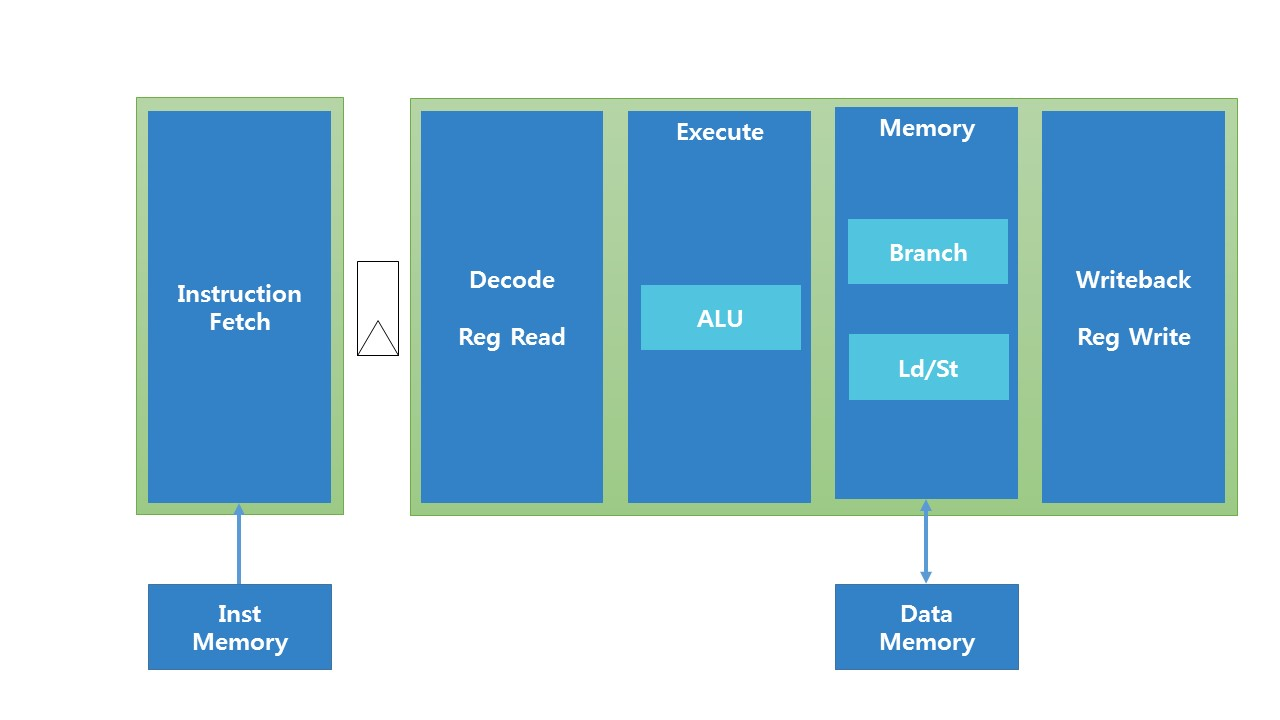
\includegraphics[scale=0.3]{twoStage.jpg}
		\caption{Two-stage Pipelined Y86-64 Processor}
		\label{fig:2pipe_proc}
	\end{center}
\end{figure}

\section{Getting Started}
\subsection{How to Download the Source Code}
Lab 5의 실습 코드를 받기 위해 수업 홈페이지에 올라와 있는 \texttt{add-lab5.sh} 스크립트를 다운받고,
이전 Lab을 수행했던 실습 디렉터리의 상위에 위치시킨 뒤 본인의 ID를 인자로 실행시킵니다.
archi16의 password(강의 홈페이지 비밀번호)와 본인의 svn 계정 비밀번호를 입력하면 실습 코드 다운이 완료됩니다.
실습 디렉터리 아래에 \texttt{lab5} 디렉터리가 새롭게 생성되었을 것입니다.

\begin{Verbatim}[frame=single]
   $ ./add-lab5.sh YOUR_ID

   archi16@hyewon.snu.ac.kr's password:

   Password for 'YOUR_ID':

   $ ls YOUR_ID/
   ... lab4/ lab5/
\end{Verbatim}


\subsection{Directory Structure of Lab 5}
Lab 5 실습의 디렉터리 구조는 다음과 같습니다.

\begin{Verbatim}[frame=single]
lab5/
    src/
        Proc.bsv
        y86
    lib/
        common-lib/
        programs/
        ...
\end{Verbatim}

\begin{description}
\item [\texttt{src/}]\hfill \ \\
	Lab 5 실습을 진행할 디렉터리입니다.

\item [\texttt{src/Proc.bsv}]\hfill \ \\
	two-stage pipeline Y86-64 프로세서가 구현되어 있는 파일입니다.

\item [\texttt{src/y86}]\hfill \ \\
	구현한 프로세서를 컴파일하고 벤치마크 프로그램을 실행할 수 있는 스크립트 파일입니다.

\item [\texttt{lib/}]\hfill \ \\
	Lab 에서 구현한 Y86-64 프로세서를 동작시키는 데 필요한 라이브러리 및 프로그램을 포함하고 있습니다.

\item [\texttt{lib/common-lib/}]\hfill \ \\
	프로세서를 구현할 때 사용되는 라이브러리 bsv 파일들입니다.

\item [\texttt{lib/programs/}]\hfill \ \\
	구현한 프로세서를 테스트하기 위한 벤치마크 프로그램들입니다.

\end{description}

\subsection{How to Simulate the Design}
Lab4에서와 같이 y86 스크립트를 통해 컴파일 및 벤치마크 프로그램 수행을 할 수 있습니다.
\subsubsection{Compiling and Simulation in Exercise}
 구현의 검증은 아래와 같이 \texttt{y86}
 스크립트를 실행하여 이뤄집니다. 
\begin{Verbatim}[frame=single]
    $ ./y86 -c 
    $ ./y86 -r
\end{Verbatim}
\noindent먼저, -c 플래그로 구현한 Y86프로세서를 컴파일을 할 수 있습니다.
다음, -r 플래그로 모든 벤치마크 수행을 테스트하거나, \texttt{-p} 플래그를 통해 특정 벤치마크 프로그램을 
테스트할 수 있습니다. 각 테스트가 끝나면, PASS 여부 및 수행한 사이클과 명령어 수,
특정 type 명령어의 수행 횟수와 Branch Prediction Miss 횟수가 출력됩니다.\\
y86 스크립트의 인자에 대한 자세한 내용은 다음과 같은 명령을 통해 확인하실 수 있습니다.
\
\begin{Verbatim}[frame=single]
./y86 -h
\end{Verbatim}

\subsubsection{Analyzing Simulation Result}
You can also see what happened in each pipeline step of each cycles.
You will find directories named as the benchmarks in the \texttt{Log} directory
after you finished running benchmark programs. The \texttt{simOut} files in these
directories contain the information on how instructions passed by each pipeline stages
while executing the corresponding benchmark. This may help your debugging.

\subsection{How to Submit Your Design}
Move into your \texttt{lab5/src} directory and type \texttt{svn commit} command.
Changed files will be uploaded to svn server.

\section{Optimizing Fetch}

The design of given processor uses two epoch registers, which was explained in the class,
to deal with control hazards that possibly occur in this pipelined processor.
This is one way to ignore the mispredicted instructions and execute only the vaild instructions.
In the rule \texttt{doFetch} of the given code, the feedback from
\texttt{execRedirect} is used to update the pc. However, the update
using \texttt{execRedirect} is somewhat inefficient and wastes a cycle.

If you successfully remove the inefficiency in the \texttt{doFetch} stage, your IPC will change like Table~\ref{table:ipcAfter}.
\begin{table}[h]
\centering
\begin{tabular}{|r|c|c|c|}
\hline
			 & Cjr & asum & bubble \\
\hline
Original IPC & 0.9 	 & 0.78  & 0.83 \\
Improved IPC & 0.9   & 0.87  & 0.91 \\
\hline
\end{tabular}
\caption{Improved IPC for Each Benchmark Programs}
\label{table:ipcAfter}
\end{table}

\noindent \paragraph{\bf Exercise 1 (20 points) :} Change the \texttt{doFetch} rule
so it does not waste a cycle. 

\section{Pipeline Y86-64 Implementation}

The provided code implementes a two-stage pipelined Y86-64 processor.
Your goal for this lab is to split one of the stages into two stages,
making the processor a three-stage pipelined implementation.
Figure~\ref{fig:3pipe_proc} shows rough sketch of what you should implement
in this lab.

\begin{figure}[htbp]
	\begin{center}
		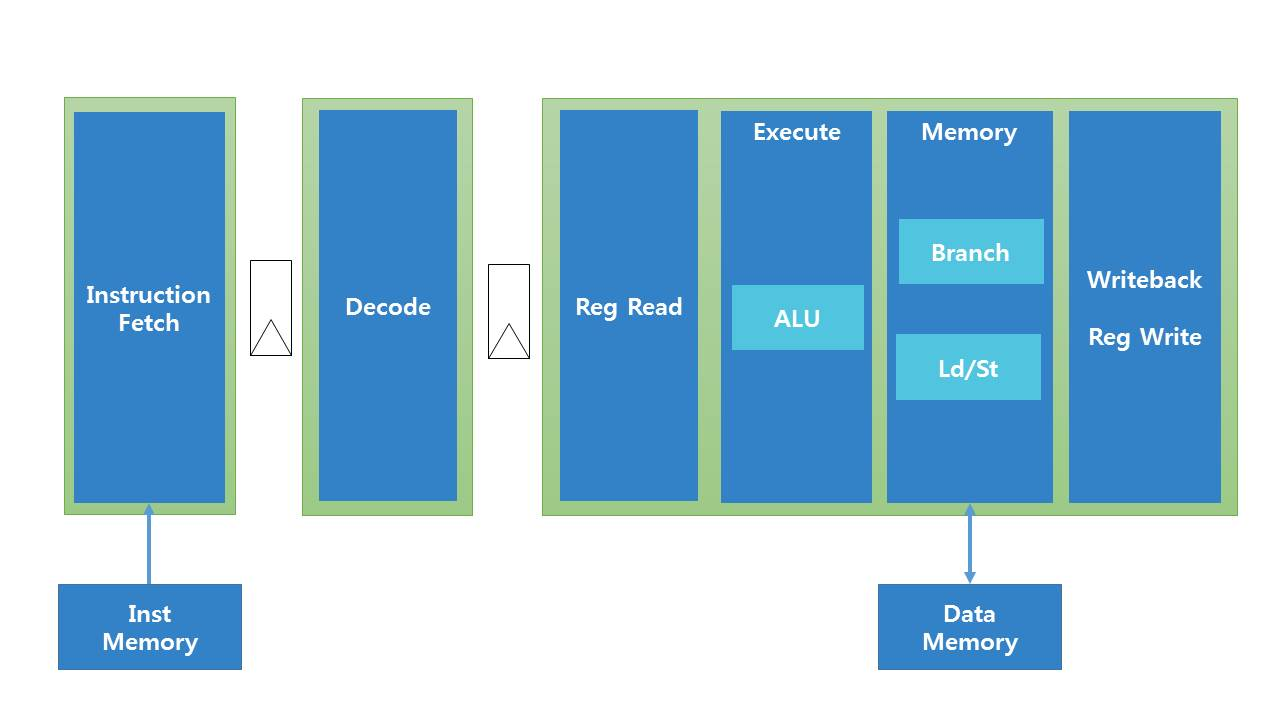
\includegraphics[scale=0.3]{threeStage.jpg}
		\caption{Three-stage Pipelined Y86-64 Processor}
		\label{fig:3pipe_proc}
	\end{center}
\end{figure}

Inside the provided \texttt{Proc.bsv} file, you can find the module
\texttt{mkProc}, which implements two rules \texttt{doFetch} and
\texttt{doRest}. Because this is a pipelined design,
these rules can be scheduled at the same time if conditions are met.
Your job is to split the \texttt{doRest} rule into two rules:
\texttt{doDecode} and \texttt{doRest}.
The \texttt{doDecode} stage should take care of \texttt{decode}.
The \texttt{doRest} stage should take care of the other part of
execution: \texttt{register read}, \texttt{execute}, \texttt{dMem} requests and writeback to \texttt{rf}.

\noindent \paragraph{\bf Exercise 2 (20 points):} Divide the
\texttt{doRest} rule into \texttt{doDecode} and \texttt{doRest},
to make the processor a three-stage pipelined implementation.
(Y86-64 구조에서 실제로는 decode와 register read가 같은 stage에서 이루어 져야 하지만, register read가 write back과 분리되면 
data hazard를 유발하므로
이번 lab에서만 decode와 register read를 분리하여 구현합니다.)

\section{Collecting Instruction Statistics}
Pipelined Processor가 가장 높은 성능을 내는 경우는 프로그램 수행의 처음과 끝 부분을 제외한
모든 cycle에서 모든 stage가 동작하고 있는 상황일 것입니다. 하지만 다양한 원인들로 인해 이러한 상황을 가지기 어려워 지는데,
그 원인들 중 하나가 Jump 또는 Call 명령어 처리 시 잘못된 pc 값 계산으로 인한 stall의 발생 입니다. 또는 일반적으로
여러 cycle이 걸리는 메모리 접근이 빈번한 프로그램의 경우, 메모리의 응답을 기다리느라 전체 수행 cycle이 증가할 수 있습니다.
\\따라서 Pipelined Processor의 성능 분석에 있어서 프로그램의 메모리 접근 비율(mrmovq, rmmovq 등 명령어의 비율) 또는 Jump 명령어 처리
시 잘못된 pc 값 사용 비율 등은 성능에 영향을 크게 미치는 중요한 요소입니다. 이와 같은 비율 정보를 얻을 수 있다면
성능 저하의 원인이 어디에서 오는지 짐작하여 적합한 최적화 방법을 도출할 수 있을 것입니다.
\\이를 위해 lab의 나머지 부분에서는 여러분이 완성한 three-stage pipeline processor에서,
benchmark를 수행하면서 명령어의 정보를 수집하는 과정을 다루도록 하겠습니다.

\subsection{How to Collect Instruction Statistics}
\texttt{mkProc} 모듈에서는 각종 수행 정보를 모으기 위해 \texttt{mkCop} 모듈을 사용하는데,
기본적으로 수행된 총 명령어 수와 cycle 수가 수집됩니다.
이렇게 수집된 정보는 benchmark 수행 완료 시 자동으로 화면에 출력됩니다.
그러나 명령어 종류별 수와 branch prediction miss 횟수는 수집하지 않고 있기 때문에 0으로 출력됩니다.

\texttt{Cop} 인터페이스에 다음과 같은 method 가 존재합니다.
\begin{Verbatim}[frame=single]
interface Cop;
  ...
  method Action incInstTypeCnt(InstCntType idx);
  method Action incBPMissCnt();
  ...
endinterface
\end{Verbatim}
\texttt{mkProc} 내에서 이 method 를 호출하여 해당하는 카운터 값을 1 만큼 증가시킬 수 있습니다.

\subsection{Counting Instructions and Address Prediction Misses}
먼저, \texttt{doRest} rule에서 현재 실행된 일부 명령어의 종류를 세는 내용을 추가합니다.
명령어의 종류를 \texttt{Control Type(call, ret, jump), Memory Type(mrmovq, rmmovq, push, pop)}
이렇게 두 가지로 구분하여, 각 명령어 종류별로 알맞은 카운터를 증가시켜야 합니다. 
위에 포함되지 않는 명령어는 카운트 하지 않습니다.
\texttt{incInstTypeCnt} method 를 이용하여 카운터를 증가시킬 수 있으며,
\texttt{InstCntType} 은 다음과 같이 정의됩니다.
\begin{Verbatim}[frame=single]
typedef enum {
	Ctr, Mem
  } InstCntType deriving(Bits, Eq);
\end{Verbatim}

다음으로, branch prediction 실패 횟수를 세는 내용을 추가합니다.
강의자료 \texttt{Lecture7 - Simple Pipelined Y86-64 Implementations}에도 나와있듯이, 
현재 구현된 processor는 가장 간단한 형태의 address prediction인 speculation을 사용하고 있습니다.
즉, jmp 같은 명령어가 오더라도 분기가 일어나지 않을 것이라고 예측하여 $pc$ 값을 항상 현재 instruction의 길이 만큼의
offset 값을 설정하여 $pc+offset$로 수정합니다.
이는 분기가 일어난 경우 예측이 틀렸다는 것을 의미하며,
분기의 발생 여부를 알 수 있는 \texttt{doRest} rule에서
상황에 따라 \texttt{incBPMissCnt} method를 호출해야 합니다.

각 벤치마크 시뮬레이션 종료 후 \texttt{mkCop} 모듈에서 수집한 각 카운터 값을
자동으로 화면에 출력하므로 결과값 출력에 대해서는 구현하지 않아도 됩니다.
정상적으로 구현된 경우 다음과 같은 결과를 얻을 수 있습니다.\\
\begin{table}[h]
\centering
\begin{tabular}{|l|c|c|c|}
\hline
\multirow{2}*{Benchmark} & \multicolumn{2}{|c|}{Instruction Types} & \multirow{2}*{BP Miss} \\
\hhline{~--~} & Ctr & Mem & \\
\hline
ctr & 1 & 1 & 0 \\
asum & 9 & 12 & 7\\
bubble & 49 & 75 & 28\\
\hline
\end{tabular}
\caption{벤치마크 별 명령어 정보 수집 결과}
\end{table}

\noindent \paragraph{\bf Exercise 3 (20 points):}
\texttt{doRest} rule에서 수행된 명령어의 수를 명령어의 종류에 따라
구하도록 구현하시오. 또한 Branch Prediction이 틀린 횟수를 세도록 구현하시오.

\end{document}
